\documentclass{amsart}
\usepackage{amsmath}
\usepackage{amssymb}
\usepackage{amsthm}
%\usepackage{MnSymbol}
\usepackage{bm}
\usepackage{accents}
\usepackage{mathtools}
\usepackage{tikz}
\usetikzlibrary{calc}
\usetikzlibrary{decorations.pathmorphing,shapes}
\usetikzlibrary{automata,positioning}
\usetikzlibrary{arrows.meta, shapes.geometric}
\usetikzlibrary{decorations.markings, fit}
\usepackage{tikz-cd}
\usepackage{forest}
\usepackage{braket} 
\usepackage{listings}
\usepackage{mdframed}
\usepackage{verbatim}
\usepackage{physics2}
\usephysicsmodule{ab,ab.legacy,diagmat,xmat}
\usepackage{derivative}
\usepackage{fixdif}
\usepackage{stmaryrd}
% \usepackage{euscript} 
% \usepackage[mathcal]{eucal}
\usepackage{stackengine} 
%\usepackage{/home/patrickl/homework/macaulay2}

%font
\usepackage[sc]{mathpazo}
\usepackage{inconsolata}
\usepackage{microtype}
% \usepackage{fontspec} 
% \setmainfont{Tex Gyre Pagella}
\usepackage[OT1,euler-digits]{eulervm}
% % \usepackage{euler-math} 
\usepackage[scaled=0.86]{berasans}
% \let\sffamilyold\sffamily
% \def\sffamily{\fontencoding{T1}\sffamilyold}
% \setmonofont{Inconsolatazi4}

%CS packages
\usepackage{algorithmicx}
\usepackage{algpseudocode}
\usepackage{algorithm}

% typeset and bib
\usepackage[english]{babel} 
% \usepackage[utf8]{inputenc} 
% \usepackage[T1]{fontenc}
% \usepackage[backend=biber,style=alphabetic,maxalphanames=4,maxnames=5,hyperref]{biblatex}
\usepackage[bookmarks, colorlinks, breaklinks]{hyperref} 
\hypersetup{linkcolor=blue,citecolor=magenta,filecolor=black,urlcolor=blue}
\usepackage{cleveref}
\usepackage{graphicx}
\graphicspath{{./}}


% other formatting packages
\usepackage{float}
\usepackage{booktabs}
\usepackage[shortlabels]{enumitem}
\setitemize{noitemsep}
\usepackage{csquotes}
%\usepackage{titlesec}
%\usepackage{titling}
%\usepackage{fancyhdr}
%\usepackage{lastpage}
% \usepackage{parskip}
\newlist{mydescription}{description}{1}
\setlist[mydescription]{style=nextline,
                        font=\bfseries,
                        % Tweak the next 4 options as needed:
                        labelindent=1cm, 
                        leftmargin =2cm,
                        rightmargin=1cm,
                        topsep     =1ex
                       }

\usepackage{lipsum}

% delimiters
\DeclarePairedDelimiter{\gen}{\langle}{\rangle}
\DeclarePairedDelimiter{\floor}{\lfloor}{\rfloor}
\DeclarePairedDelimiter{\ceil}{\lceil}{\rceil}


\newtheorem{thm}{Theorem}[section]
\newtheorem{cor}[thm]{Corollary}
\newtheorem{prop}[thm]{Proposition}
\newtheorem{lem}[thm]{Lemma}
\newtheorem{conj}[thm]{Conjecture}
\newtheorem{quest}[thm]{Question}
\newtheorem{claim}[thm]{Claim}

\theoremstyle{definition}
\newtheorem{defn}[thm]{Definition}
\newtheorem{defns}[thm]{Definitions}
\newtheorem{con}[thm]{Construction}
\newtheorem{exm}[thm]{Example}
\newtheorem{exms}[thm]{Examples}
\newtheorem{notn}[thm]{Notation}
\newtheorem{notns}[thm]{Notations}
\newtheorem{addm}[thm]{Addendum}
\newtheorem{exer}[thm]{Exercise}

\theoremstyle{remark}
\newtheorem{rmk}[thm]{Remark}
\newtheorem{rmks}[thm]{Remarks}
\newtheorem{warn}[thm]{Warning}
\newtheorem{sch}[thm]{Scholium}


% unnumbered theorems
\theoremstyle{plain}
\newtheorem*{thm*}{Theorem}
\newtheorem*{prop*}{Proposition}
\newtheorem*{lem*}{Lemma}
\newtheorem*{cor*}{Corollary}
\newtheorem*{conj*}{Conjecture}

% unnumbered definitions
\theoremstyle{definition}
\newtheorem*{defn*}{Definition}
\newtheorem*{exer*}{Exercise}
\newtheorem*{defns*}{Definitions}
\newtheorem*{con*}{Construction}
\newtheorem*{exm*}{Example}
\newtheorem*{exms*}{Examples}
\newtheorem*{notn*}{Notation}
\newtheorem*{notns*}{Notations}
\newtheorem*{addm*}{Addendum}


\theoremstyle{remark}
\newtheorem*{rmk*}{Remark}

% shortcuts
\newcommand{\Ima}{\mathrm{Im}}
\newcommand{\A}{\mathbb{A}}
\newcommand{\G}{\mathbb{G}}
\newcommand{\N}{\mathbb{N}}
\newcommand{\R}{\mathbb{R}}
\newcommand{\C}{\mathbb{C}}
\newcommand{\Z}{\mathbb{Z}}
\newcommand{\Q}{\mathbb{Q}}
\newcommand{\E}{\mathbb{E}}
\renewcommand{\k}{\Bbbk}
\renewcommand{\L}{\mathbb{L}}
\renewcommand{\P}{\mathbb{P}}
\newcommand{\M}{\mathcal{M}}
\newcommand{\Mbar}{\overline{\mathcal{M}}}
\newcommand{\g}{\mathfrak{g}}
\newcommand{\h}{\mathfrak{h}}
\newcommand{\n}{\mathfrak{n}}
\renewcommand{\b}{\mathfrak{b}}
\newcommand{\ep}{\varepsilon}
\newcommand*{\dt}[1]{%
   \accentset{\mbox{\Huge\bfseries .}}{#1}}
%\renewcommand{\abstractname}{Official Description}
\newcommand{\mc}[1]{\mathcal{#1}}
% \newcommand{\msc}[1]{\mathscr{#1}}
\newcommand{\T}{\mathbb{T}}
\newcommand{\mf}[1]{\mathfrak{#1}}
\newcommand{\mbf}[1]{\mathbf{#1}}
\newcommand{\bv}{\mbf{v}}
\newcommand{\bq}{\mbf{q}}
\newcommand{\bp}{\mbf{p}}
\newcommand{\btau}{\bm{\tau}}
\newcommand{\mr}[1]{\mathrm{#1}}
\newcommand{\on}[1]{\operatorname{#1}}
\newcommand{\ms}[1]{\mathsf{#1}}
\newcommand{\mt}[1]{\mathtt{#1}}
\newcommand{\ol}[1]{\overline{#1}}
\newcommand{\ul}[1]{\underline{#1}}
\newcommand{\wt}[1]{\widetilde{#1}}
\newcommand{\wh}[1]{\widehat{#1}}
\renewcommand{\div}{\operatorname{div}}
\newcommand{\1}{\mathbf{1}}
\newcommand{\2}{\mathbf{2}}
\newcommand{\3}{\mathbf{3}}
\newcommand{\I}{\mathrm{I}}
\newcommand{\II}{\mr{I}\hspace{-1.3pt}\mr{I}}
\newcommand{\III}{\mr{I}\hspace{-1.3pt}\mr{I}\hspace{-1.3pt}\mr{I}}
\renewcommand{\v}{\mbf{v}}
\newcommand{\w}{\mbf{w}}
\newcommand{\bmu}{\bm{\mu}}
\newcommand{\pre}{\mr{pre}}
\newcommand{\vir}{\mr{vir}}
\newcommand{\fl}{\mr{fl}}
\newcommand{\ps}[1]{\llbracket #1 \rrbracket}
\newcommand{\ls}[1]{\llparenthesis #1 \rrparenthesis}
\newcommand{\GL}{\mr{GL}}
\newcommand{\SL}{\mr{SL}}
\newcommand{\SO}{\mr{SO}}
\newcommand{\Sp}{\mr{Sp}}
\newcommand{\gl}{\mf{gl}}
\renewcommand{\sl}{\mf{sl}}
\newcommand{\so}{\mf{so}}
\renewcommand{\sp}{\mf{sp}}

\DeclareMathOperator{\Der}{Der}
\DeclareMathOperator{\Tor}{Tor}
\DeclareMathOperator{\Hom}{Hom}
\DeclareMathOperator{\End}{End}
\DeclareMathOperator{\Ext}{Ext}
\DeclareMathOperator{\ad}{ad}
\DeclareMathOperator{\Ad}{Ad}
\DeclareMathOperator{\Aut}{Aut}
\DeclareMathOperator{\Rad}{Rad}
\DeclareMathOperator{\Pic}{Pic}
\DeclareMathOperator{\NS}{NS}
\DeclareMathOperator{\supp}{supp}
\DeclareMathOperator{\Supp}{Supp}
\DeclareMathOperator{\depth}{depth}
\DeclareMathOperator{\sgn}{sgn}
\DeclareMathOperator{\spec}{Spec}
\DeclareMathOperator{\Spec}{Spec}
\DeclareMathOperator{\proj}{Proj}
\DeclareMathOperator{\Proj}{Proj}
\DeclareMathOperator{\ord}{ord}
\DeclareMathOperator{\Div}{Div}
\DeclareMathOperator{\Bl}{Bl}
\DeclareMathOperator{\coker}{coker}
\DeclareMathOperator{\ev}{ev}
\DeclareMathOperator{\st}{st}
\DeclareMathOperator{\pr}{pr}
\DeclareMathOperator{\ch}{ch}
\DeclareMathOperator{\Cont}{Cont}

% \addbibresource{../../notes/math.bib}

\title{Topics in Geometric Representation Theory}
\author{Lectures by Xin Jin \\ Notes by Patrick Lei}
\date{Spring 2026}
\allowdisplaybreaks

\begin{document}
    
\begin{abstract}
    The goal of this course is to introduce many geometric objects and tools that are in the heart of GRT. Below is the tentative plan of the course:
    \begin{itemize}
        \item Part I.  I will talk about the geometry of complex semisimple Lie algebras and groups.
        Specific topics include 
            \begin{enumerate}[(1)]
                \item The geometry of flag variety, nilpotent cone, Grothendieck-Springer resolution, Steinberg variety and an introduction to Springer theory
                \item The wonderful compactification of semisimple groups and more general toroidal compactifications of reductive groups.
            \end{enumerate}
        We will follow some standard text/notes (and some additional references):
        \begin{itemize}
            \item Chriss-Ginzburg, \textit{Representation theory and complex geometry}, mostly chapter 3 and part of chapter 2
            \item Evens-Jones, \textit{On the wonderful compactification}
        \end{itemize}
        \item Part 2. We will focus on a class of completely integrable systems, called the universal centralizers $J_G$ (or under other names: Toda systems, regular centralizer group schemes, or bi-Whittaker reductions), associated with a semisimple (or reductive) group $G$.
        This class of completely integrable systems lies at the crossroads of many different subjects in differential geometry, GRT (including geometric Langlands), (homological and enumerative) mirror symmetry, and mathematical physics (e.g. the class of Coulomb branches).
        Selected topics include:
        \begin{enumerate}[(1)]
            \item A partial log-compactification of $J_G$, by Balibanu (as an application of (2) in part 1)
            \item Symplectic geometry of $J_G$ and sketch of its homological mirror symmetry (based on some of my recent work)
            \item Depending on interest, I will sketch the proof of a hyperKahler metric on it constructed from gauge theory (following Donaldson, Kronheimer and Bielawski).
        \end{enumerate}
    \item Prerequisite: Basic knowledge of differential topology and complex geometry is assumed. Familiarity with semisimple Lie algebras and algebraic groups, as well as their representations, will be helpful but is not strictly required. We will follow the approach of Chriss–Ginzburg in recalling and supplementing the necessary background as needed.
    \end{itemize}
\end{abstract}

\maketitle

\tableofcontents

\section{Introduction}%
\label{sec:introduction}

Representation theory studies some group $G$ with some structure by considering representations \((V,\rho \colon G \to \on{GL}(V))\) where $V$ is a vector space and \(\rho\) is a group homomorphism with suitable properties. This seems like a purely algebraic question, but it is already very hard even when \(G\) is a finite group (in the nonabelian case). We may now bring in various geometric methods to construct representations of $G$:
\begin{enumerate}
    \item If $G$ acts on an algebraic variety \(X\), then there is an action of $G$ on the space of functions on $X$;
    \item If $G$ acts on an algebraic variety \(X\), then we may consider a $G$-equivariant line bundle $\mc{L}$ on $X$ (which is a line bundle on $[X/G]$), we may consider the cohomology groups \(H^i(X,\mc{L})\) which are representations of $G$. If \(X\) is projective, then these cohomology groups are finite-dimensional;
    \item If \(G\) acts on $X$, then it also acts on the cohomology \(H^{\bullet}(X) \)  for any generalized cohomology theory;
    \item There are also more hidden and subtle symmetries, where instead of actual group actions, we consider correspondences acting on cohomology groups. We will see examples of this later when we discuss Springer theory. In addition, we can lift this to the level of derived categories and consider Fourier-Mukai transforms;
\end{enumerate}

\subsection{Overview of the course}%
\label{sub:Overview of the course}


The first part of the course will focus on the basics of geometric representation theory, largely focusing on Springer theory, the Borel-Weil-Bott theorem, and the geometry of the wonderful compactification \(\ol{G}\).

The second part of the course will focus on a completely integrable system called the Toda system and its homological mirror symmetry. One motivation for this is the notion of categorification, for example going from the Hecke algebra to the Hecke category, which will turn out to be a category of constructible sheaves. 

One origin of categorification in algebraic geometry is Grothendieck's function-sheaf correspondence, which we will adapt to our setting (in particular, we will not need \(\ell\)-adic sheaves). One particularly simple example of this is upgrading the integers $\Z$ to the derived category of vector spaces over a field $k$, where the original integer is recovered as the Euler characteristic.

For a more sophisticated example, we may consider a smooth manifold $X$ with a stratification $\mc{S} = \ab\{S_{\alpha} \}$ by locally closed submanifolds. We may consider the space $\ms{Fun}_{\mc{S}}(X)$ of constructible functions (taking values in integers) with respect to \(\mc{S}\), which are locally constant on each stratum \(S_{\alpha}\). The natural categorification of this is the derived category \(\ms{Sh}_{\mc{S}}(X)\)  of constructible sheaves on $X$, where all cohomology sheaves are locally constant on each stratum \(S_{\alpha}\). The original constructible function is recovered by taking the Euler characteristic of the stalk at each point. In addition, we may recover the functions as
\[ K_0(\ms{Sh}_{\mc{S}}(X)) \cong \ms{Fun}_{\mc{S}} (X). \]

\subsection{Homological mirror symmetry}%
\label{sub:Homological mirror symmetry}

We will now discuss a connection to symplectic geometry. If we have a stratification \(\mc{S}\), then we may consider the union
\[ T^*_{\mc{S}}X \coloneqq \bigsqcup_{S_{\alpha} \in \mc{S}} T^*_{S_{\alpha}} X \]
of conormal bundles to the strata and consider the microlocal sheaf theory. In particular, each constructible sheaf $\mc{F}$ has a microlocal stalk at each $(x, \xi) \in T^*_{\mc{S}}X$ as in~\Cref{fig:microlocal_stalk}. For example, if we have a restriction map $\mc{F}(U) \to \mc{F}(V)$, then the microlocal stalk is
\[ \mu_{(x, \xi)}(\mc{F}) = \on{Cone}(\mc{F}(U) \to \mc{F}(V))[\cdots], \]
where the shift is not canonical. One upshot of this approach is that
\[ K_0(\ms{Sh}_{\mc{S}}(X)) \cong \ms{Fun}_{\mc{S}} (X) \cong H_{\mr{top}}^{\mr{BM}}(T_{\mc{S}}^* X). \]
\begin{figure}[htpb]
\begin{center}
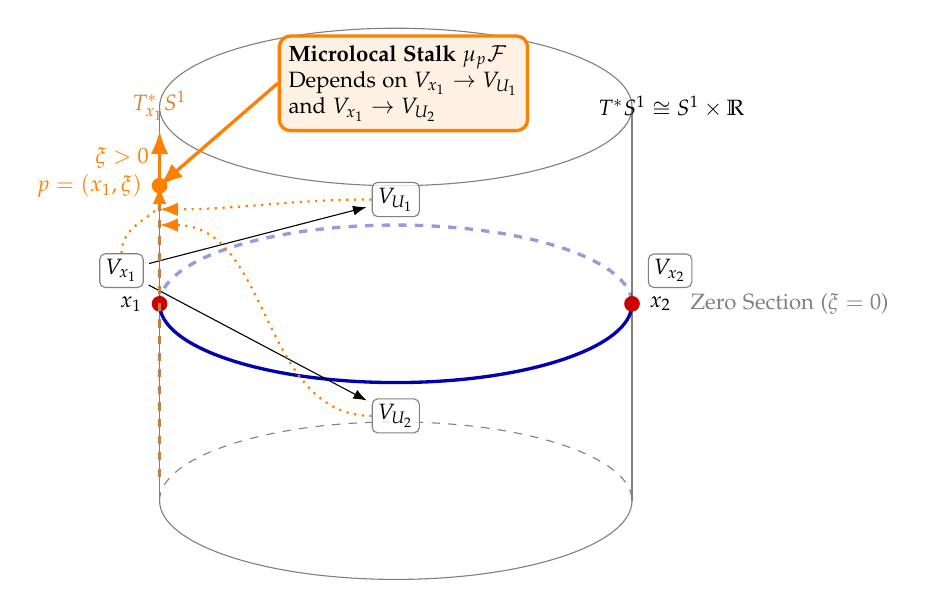
\begin{tikzpicture}[
    font=\footnotesize,
    >=Latex,
    % Define geometric parameters for the cylinder perspective
    x_rad/.style={x radius=3cm},
    y_rad_main/.style={y radius=1cm},
    y_rad_cap/.style={y radius=1cm},
    cylinder_height/.store in=\cylht, cylinder_height=2.5cm,
    % Define styles for strata and data
    stratum_point/.style={circle, fill=red!80!black, inner sep=2pt, outer sep=0pt},
    stratum_line/.style={very thick, blue!70!black},
    sheaf_data/.style={fill=white, fill opacity=0.8, text opacity=1, draw=gray, thin, rounded corners=2pt, inner sep=2pt},
    micro_point/.style={circle, fill=orange, inner sep=2pt},
    conormal_fiber/.style={thick, orange!50!gray, dashed}
]

% --- 1. Draw the Cylinder (Cotangent Bundle T*S^1) ---

% Bottom cap (back half dashed)
\draw[gray, dashed, x_rad, y_rad_cap] (-3,-\cylht) arc (180:0:3cm and 1cm);
\draw[gray, x_rad, y_rad_cap] (-3,-\cylht) arc (180:360:3cm and 1cm);

% Vertical walls
\draw[gray] (-3, -\cylht) -- (-3, \cylht);
\draw[gray] (3, -\cylht) -- (3, \cylht);

% Top cap
\draw[gray, x_rad, y_rad_cap] (0,\cylht) circle (3cm and 1cm);

% Label the spaces
\node at (3.5, \cylht) {$T^*S^1 \cong S^1 \times \mathbb{R}$};
\node[gray] at (5.0, 0) {Zero Section ($\xi=0$)};


% --- 2. Draw the Stratified Base Space S^1 (Zero Section) ---

% Define coordinates for the stratifying points
\coordinate (x1) at (-3, 0);
\coordinate (x2) at (3, 0);

% Interval U1 (Back semi-circle)
\draw[stratum_line, opacity=0.4, dashed, x_rad, y_rad_main] 
    (x1) arc (180:0:3cm and 1cm);
\coordinate (u1_mid) at (0, 0.9); % Midpoint for label

% Interval U2 (Front semi-circle)
\draw[stratum_line, x_rad, y_rad_main] 
    (x1) arc (180:360:3cm and 1cm);
\coordinate (u2_mid) at (0, -0.9); % Midpoint for label

% Points x1 and x2
\node[stratum_point, label={left:$x_1$}] at (x1) {};
\node[stratum_point, label={right:$x_2$}] at (x2) {};


% --- 3. Visualize Sheaf Data on the Base ---

% Stalks at points
\node[sheaf_data, anchor=south east] (Vx1) at ($(x1)+(-0.2,0.2)$) {$V_{x_1}$};
\node[sheaf_data, anchor=south west] (Vx2) at ($(x2)+(0.2,0.2)$) {$V_{x_2}$};

% Stalks on intervals
\node[sheaf_data, anchor=south] (Vu1) at ($(u1_mid)+(0,0.2)$) {$V_{U_1}$};
\node[sheaf_data, anchor=north] (Vu2) at ($(u2_mid)+(0,-0.3)$) {$V_{U_2}$};

% Draw restriction/generization maps (sp)
% From x1 to U1 and U2
\draw[->, shorten >=2pt, shorten <=2pt] (Vx1) -- (Vu1);
\draw[->, shorten >=2pt, shorten <=2pt] (Vx1) -- (Vu2);
% From x2 to U1 and U2 (optional, for completeness)
%\draw[->, shorten >=2pt, shorten <=2pt, opacity=0.5] (Vx2) -- (Vu1);
%\draw[->, shorten >=2pt, shorten <=2pt, opacity=0.5] (Vx2) -- (Vu2);


% --- 4. Visualize the Microlocal Stalk ---

% Draw the conormal fiber over x1 (T^*_{x1} S^1)
\draw[conormal_fiber] (-3, -2.2) -- (-3, 2.2) node[above, orange!70!gray] {$T^*_{x_1}S^1$};

% Pick a point p = (x1, xi) with xi > 0
\coordinate (p) at (-3, 1.5);
\node[micro_point] at (p) {};

% Add cotangent vector xi indicating direction
\draw[->, very thick, orange] (p) -- ++(0, 0.7) node[midway, left] {$\xi > 0$};
\node[left, orange] at ($(p)-(0.1,0)$) {$p=(x_1, \xi)$};

% Label the microlocal stalk
% We use a callout box to indicate it depends on local data
\node[draw=orange, very thick, fill=orange!10, rounded corners, align=left, anchor=west] 
    (micro_label) at (-1.5, 2.8) 
    {\textbf{Microlocal Stalk} $\mu_p\mathcal{F}$\\
     Depends on $V_{x_1} \to V_{U_1}$ \\
     and $V_{x_1} \to V_{U_2}$};

\draw[orange, very thick, ->] (micro_label.west) -- (p);

% Add visual connectors showing dependence
% Connecting the base data to the microlocal point to show the relationship
\draw[orange, dotted, thick, ->] (Vx1.north) to[out=90, in=270] (p);
\draw[orange, dotted, thick, ->] (Vu1.west) to[out=180, in=0] ($(p)+(0,-0.3)$);
\draw[orange, dotted, thick, ->] (Vu2.west) to[out=180, in=0] ($(p)+(0,-0.5)$);

\end{tikzpicture}
\end{center}
\caption{A microlocal stalk}%
\label{fig:microlocal_stalk}
\end{figure}


The following theorem inspired many subsequent works, including the lecturer's PhD work.
\begin{thm}[Nadler-Zaslow]
    The dg-category $\ms{Sh}_c(X)$ of constructible sheaves on $X$ equivalent the Fukaya category \(\ms{Fuk}(T^* X)\) of the cotangent bundle \(T^* X\) of $X$.
\end{thm}
We will now discuss a geometric interpretation. We may consider the characteristic cycle $\on{CC}(\mc{F})$ of a constructible sheaf, which is a conic Lagrangian cycle in \(T^* X\). However, the objects of the Fukaya category are smooth Lagrangian submanifolds with the cochain complexes of morphisms being given by counting interesection points and holomorphic polygons. See~\Cref{fig:fukaya} for a visualization. It is usually very difficult to calculate the Fukaya category directly, but the theorem allows us to translate these questions into questions about constructible sheaves, which are more manageable.
\begin{figure}[htpb]
\begin{center}
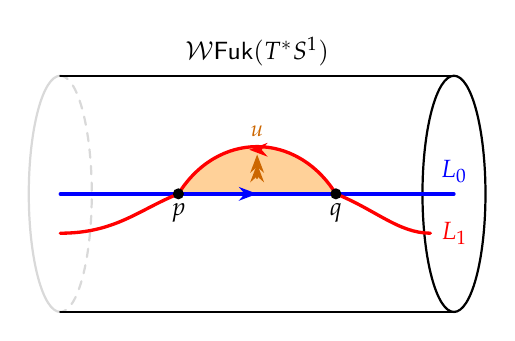
\begin{tikzpicture}[
    >=Stealth,
    font=\small,
    line cap=round,
    line join=round
]

% --- Definitions ---
\def\cylLen{6}   % Length of cylinder
\def\cylRad{1.5} % Radius of cylinder
\def\xStart{0.5}
\def\xEnd{5.5}

% --- Draw Back of Cylinder (Inside) ---
\draw[gray!30, thick] (\xStart, \cylRad) arc (90:270:0.4 and \cylRad);
\draw[gray!30, thick, dashed] (\xStart, \cylRad) arc (90:-90:0.4 and \cylRad);

% --- Draw Cylinder Body ---
% Top and Bottom lines
\draw[thick] (\xStart, \cylRad) -- (\xEnd, \cylRad);
\draw[thick] (\xStart, -\cylRad) -- (\xEnd, -\cylRad);

% Right Cap (Front)
\draw[thick] (\xEnd, 0) ellipse (0.4 and \cylRad);

% --- Define Lagrangians ---

% L0: The Zero Section (Straight horizontal line along the "front" face)
% We place it slightly offset in z-space conceptually, but y=0 in 2D
\coordinate (L0_start) at (\xStart, 0);
\coordinate (L0_end) at (\xEnd, 0);

% L1: An oscillating Lagrangian (e.g., graph of df or a wrapped curve)
% It creates a "Bigon" (two intersection points)
\coordinate (p) at (2, 0); % Intersection 1
\coordinate (q) at (4, 0); % Intersection 2

% --- Draw the Holomorphic Polygon (Shading) ---
% We fill the area between L0 and L1 between p and q
\fill[orange!90!yellow, opacity=0.4] 
    (p) 
    -- (2.2, 0) % Guide point along L0
    -- (q) 
    .. controls (3.5, 0.8) and (2.5, 0.8) .. (p);

% Add a flow arrow inside the polygon to indicate holomorphic map u
\draw[->, orange!80!black, thick, decoration={markings, mark=at position 0.6 with {\arrow{>}}}, postaction={decorate}] 
    (3, 0.2) -- (3, 0.5) node[above=0.1, font=\footnotesize] {$u$};

% --- Draw L0 (Blue) ---
\draw[blue, very thick] (L0_start) -- (L0_end) node[above] {$L_0$};

% --- Draw L1 (Red) ---
% Curve starts low, intersects p, goes high, intersects q, goes low
\draw[red, very thick] 
    (\xStart, -0.5) 
    .. controls (1.2, -0.5) and (1.5, -0.2) .. (p)
    .. controls (2.5, 0.8) and (3.5, 0.8) .. (q)
    .. controls (4.5, -0.2) and (4.8, -0.5) .. (5.2, -0.5)
    node[right] {$L_1$};

% --- Draw Intersection Points ---
\fill[black] (p) circle (2pt) node[below] {$p$};
\fill[black] (q) circle (2pt) node[below] {$q$};

% --- Annotations ---
\node[above] at (3, \cylRad) {$\mathcal{W}\ms{Fuk}(T^*S^1)$};

% Optional: Draw vector field or boundary orientation on the strip
% Top boundary orientation
\draw[->, red, thick] (3, 0.56) -- (2.9, 0.56); 
% Bottom boundary orientation
\draw[->, blue, thick] (2.9, 0) -- (3, 0);

\end{tikzpicture}
\end{center}
\caption{Two objects in the Fukaya category}%
\label{fig:fukaya}
\end{figure}


\begin{proof}[Sketch of proof]
    We will begin by discussing why there is a fully faithful functor \(\on{Sh}_c(X) \to \ms{Fuk}(T^* X)\). The first step is to find some nice generators of the constructible sheaf category. For this, we consider open embeddings $j \colon U \hookrightarrow X$ and extension by zero $j_! \C_U$ of the constant sheaf on $U$. These have characteristic cycles given by the conormal bundle to the boundary \(\partial U\) (together with the zero section at $U$). We will send this sheaf $j_! \C_U$ to a smoothing of its characteristic cycle, as depicted in~\Cref{fig:charcycle_smoothing}.
    \begin{figure}[htpb]
    \begin{center}
    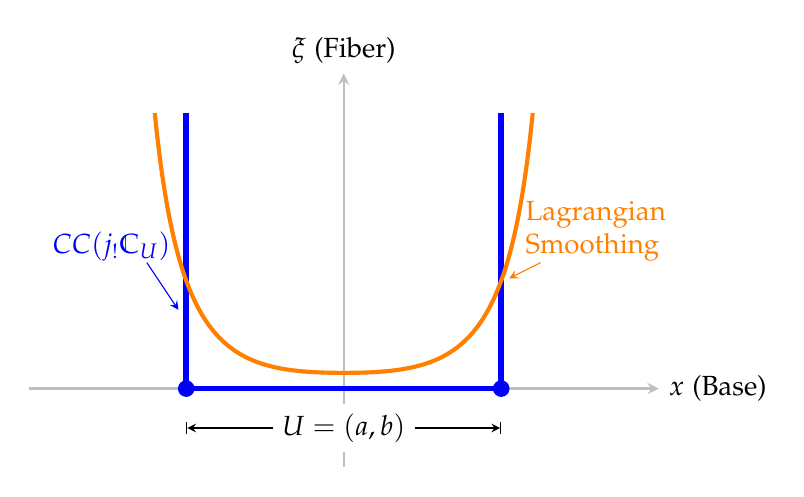
\begin{tikzpicture}[>=stealth, thick]

    % --- 1. Axes (T*R plane) ---
    \draw[->, gray!50] (-4, 0) -- (4, 0) node[right, black] {$x$ (Base)};
    \draw[->, gray!50] (0, -1) -- (0, 4) node[above, black] {$\xi$ (Fiber)};

    % Define Interval U = (-2, 2)
    \def\a{-2}
    \def\b{2}

    % --- 2. Singular Characteristic Cycle CC(F) ---
    % F = j_! C_U (Extension by zero)
    % Cycle = Zero section over U + Conormals at boundary
    % Drawn in BLUE
    
    % The Zero Section part: U x {0}
    \draw[blue, line width=2pt] (\a, 0) -- (\b, 0);
    
    % The Conormal parts: {a} x R+ and {b} x R+ (Upward orientation for visual standard)
    \draw[blue, line width=2pt] (\a, 0) -- (\a, 3.5);
    \draw[blue, line width=2pt] (\b, 0) -- (\b, 3.5);
    
    % Draw "Nodes" at the singularities (corners)
    \fill[blue] (\a, 0) circle (3pt);
    \fill[blue] (\b, 0) circle (3pt);


    % --- 3. Lagrangian Smoothing ---
    % A smooth approximation that rounds the corners
    % Drawn in ORANGE
    
    \draw[orange, line width=1.5pt] 
        (\a - 0.4, 3.5) 
        .. controls (\a - 0.1, 0.5) and (\a + 0.5, 0.2) .. (0, 0.2) % Left corner smoothing
        .. controls (\b - 0.5, 0.2) and (\b + 0.1, 0.5) .. (\b + 0.4, 3.5); % Right corner smoothing


    % --- 4. Annotations ---
    
    % Label the Interval U
    \draw[|<->|, thin, black] (\a, -0.5) -- (\b, -0.5) node[midway, fill=white] {$U = (a,b)$};
    
    % Label the Singular Cycle
    \node[blue, align=left] at (-2.95, 1.8) {$CC(j_! \mathbb{C}_U)$};
    \draw[->, blue, thin] (-2.5, 1.6) -- (-2.1, 1);
    
    % Label the Smoothing
    \node[orange, align=left] at (3.2, 2) {Lagrangian\\Smoothing};
    \draw[->, orange, thin] (2.5, 1.6) -- (2.1, 1.4);

\end{tikzpicture}
    \end{center}
    \caption{Characteristic cycle and its smoothing}%
    \label{fig:charcycle_smoothing}
    \end{figure}
    

    To prove essential surjectivity, all of the Hom complexes in the Fukaya category can be calculated using Morse theory. For more details, see the original paper by Nadler-Zaslow.
\end{proof}

One reason to consider the Fukaya category is homological mirror symmetry, which was originally proposed by Kontsevich. For certain symplectic manifolds $M$, there is a \textit{mirror partner} \(\check{M}\), which is a complex algebraic variety, and Kontsevich conjectured that there is an equivalence of categories
\[ \ms{Fuk}(M) \simeq \ms{Coh}(\check{M}). \]
The simplest example is when \(M = T^* S^1\), where we need to consider the fully wrapped Fukaya category. We have an equivalence
\[ \mc{W}\ms{Fuk}(T^* S^1) \simeq \ms{Loc}(S^1) \]
(modulo technical details), but the upshot is that all characteristic cycles are supported inside the zero section. Local systems are on \(S^1\) are simply representations of \(\pi_1(S^1) \cong \Z\), which are simply modules over the group algebra \(\C[\Z] \cong \C[t, t^{-1}] = \mc{O}(\C^{\times})\). Ignoring finiteness conditions, these are simply quasicoherent sheaves on \(\C^{\times}\).

\begin{rmk}
    For the purposes of representation theory, we will treat $\pi_1(S^1) = \mathbb{X}_{\bullet}(S^1)$ as cocharacters, which will be identified with the characters $\mathbb{X}^{\bullet}(\C^{\times})$ on the mirror side. This picture generalizes if we consider algebraic tori of any rank and is a version of Langlands duality in the abelian case.
\end{rmk}

\begin{rmk}
    Homological mirror symemtry is closely related to the geometric Langlands correspondence, where we send the Hitchin system for $G$ to the character variety for the Langlands dual group \(G^{\vee}\). There are some technical issues, but the Betti geometric Langlands correspondence is essentially homological mirror symmetry here.
\end{rmk}

One modification of this is to complexify the Fukaya side into $T^* T$, and in this case the (appropriate version of the) wrapped Fukaya category  still reduces to local systems on $T$. Traditionally, we considered $T^* T_c$ (the cotangent bundle of the compact form) because of the SYZ mirror symmetry philosophy, which predicts that a manifold $M$ and its mirror $\check{M}$ have dual Lagrangian torus fibrations. In general, it is very hard to use SYZ to construct mirrors because there are usually singular fibers, which are hard to control.

However, one way to produce a mirror is to believe in homological mirror symmetry and then try to find a variety $\check{M}$ such that
\[ \ms{Fuk}(M) \simeq \ms{Coh}(\check{M}). \]
If the fibration has a Lagrangian section, then each smooth fiber becomes a Lie group, so $\ms{Fuk}(M)$ is expected to pick up a ``convolution'' symmetric monoidal structure, which should correspond to the tensor product of coherent sheaves in some kind of non-linear Fourier transform.

In the second part of the course, we will generalize the duality $T^*T \leftrightarrow T^{\vee}$ to the universal centralizer (or Toda system) $J_G$, where $G$ is a semisimple complex Lie group. This is related to representation theory for two reasons.
\begin{itemize}
    \item $J_G$ is also called the bi-Whittaker reduction and represents something like the generic part of the representation of $G$, namely the ``commutative part'' of the Hecke category;
    \item If we add a loop to $G$, then we obtain the affine Toda system;
    \item There is a partial (log) compactification $\ol{J}_G^{\log}$ over the base $\g^* \sslash G$ constucted by Balibanu whose fibers are a kind of regular Hessenberg variety (a generalization of Springer fibers). The central fiber is the Peterson variety $Y_P$, which is a closed subvariety of the flag variety $G/B$ and is related to the quantum cohomology of $G^{\vee}/P^{\vee}$ via the isomorphism
    \[ QH^*(G^{\vee} / P^{\vee}) \cong \mc{O}(Y_P). \]
\end{itemize}

\part{Geometry of complex semisimple Lie algebras and groups}

\section{Review of semisimple Lie algebras/groups}%
\label{sec:Review of semisimple Lie algebras/groups}

Eventually, the groups we are interested in are $\on{SL}_n(\C)$, $\on{SO}_n(\C)$, and $\on{Sp}_{2n}(\C)$ with Lie algebras $\mf{sl}_n(\C)$, $\so_n(\C)$, and $\sp_{2n}(\C)$. However, along the way we will encounter groups like Borels and unipotent groups.

Every Lie group has both a left and right action of $G$ on itself given by the multiplication map
\[ m \colon G \times G \to G. \]
We may consider the tangent space $\g = T_e G$ at the identity, and left translation of vector fields gives an isomorphism
\[ L \colon G \times \g \xrightarrow{\sim} TG \qquad (g, \xi) \mapsto L_{g *} \xi. \]
The right action gives another trivialization
\[ R \colon G \times \g \xrightarrow{\sim} TG \qquad (g, \xi) \mapsto R_{g^{-1} *} \xi. \]
These two are related by the diagram
\begin{equation*}
\begin{tikzcd}
    G \times \g \ar{r}{L} \ar[swap]{d}{\iota \times (-1)} & TG \ar{d}{T\iota} \\
    G \times \g \ar{r}{R} & TG,
\end{tikzcd}
\end{equation*}
where $\iota$ is the map sending an element of $G$ to its inverse. If we fix $\xi \in \g$, then applying $L$ gives us a left-invariant vector field $\xi^{\ell}$ on $G$, and similarly applying $R$ gives a right-invariant vector field $\xi^r$. 

\begin{lem}\leavevmode
    \begin{enumerate}
        \item Left (resp. right) invariant vector fields on $G$ are closed under the Lie bracket;
        \item The left and right-invariant vector fields induce the same Lie bracket on $\g$.
    \end{enumerate}
\end{lem}

The main idea of the proof is that the Lie bracket is preserved by diffeomorphisms and in particular left (or right) translation. 

\begin{rmk}
    If we have any action $a \colon G \times X \to X$, then taking the derivative
    \[ (\d{a})_e \colon \g \times X \to X \]
    gives an infinitesimal action of $G$ on $X$ (as in a map from $\g$ to vector fields on $X$). For example, $L$ is simply 
    \[ (\d{m})_{e, \text{factor 2}} \colon G \times \g \to TG \]
    and a similar statement is true for $R$.
\end{rmk}

One important action of $G$ on itself is the \textit{adjoint action}, where $G$ acts on itself by conjugation. On the tangent space, we have $(R_{g^{-1}})_* L_{g*} = L_{g*} (R_{g^{-1}})_*$. By definition, we now have
\[ \Ad_g \xi \coloneqq (R_{g^{-1}})_* L_{g*} \xi, \]
which induces a map
\[ \Ad \colon G \to \GL(\g). \]
Therefore, another equivalent definition of the Lie bracket is to simply differentiate the adjoint action. There is also an exponential map $\exp \colon \g \to G$, and the Lie bracket is defined as
\[ [\xi, \eta] \coloneqq \eval{\odv{}{t}}_{t=0} \Ad_{\exp(t\xi)} \eta. \]

\begin{rmk}
    Any finite-dimensional abstract Lie algebra is isomorphic to a subalgebra of $\gl_n$ by Ado's theorem, which says that every finite-dimensional Lie algebra has a finite-dimensional faithful representation. In particular, every finite-dimensional Lie group over $\R$ is locally an immersed subgroup of $\GL_n(\R)$ for some $n$.
\end{rmk}

We will give some principles of Lie theory:
\begin{itemize}
    \item The Lie group is (up to taking its universal cover) determined by its Lie algebra. Given a connected Lie group $(H, e)$, then any discrete covering $(H', e')$ inherits a unique group structure whose kernel lies in the center of $H'$ (this works because the fundamental group of $H$ is abelian due to the group structure). Conversely, any discrete central quotient of $H$ is a Lie group with the same Lie algebra. If we work analytically, $H$ has a universal cover, which is the unique simply connected Lie group with the same Lie algebra as $H$.
    \item If $G$ and $H$ are Lie groups such that $G$ is connected, then any Lie group homomorphism
    \[ \rho \colon G \to H \]
    is uniquely determined by its derivative $\d{\rho} \colon \g \to \mf{h}$, which is a Lie algebra homomorphism.
    \item For $\g = \on{\ms{Lie}} G$ and any embedding $\mf{h} \hookrightarrow \g$, the subgroup of $G$ generated by $\exp(\mf{h})$ is an immersed Lie subgroup of $G$ with Lie algebra $\mf{h}$.
\end{itemize}

By Ado's theorem, we see that the embedding $\g \hookrightarrow \gl_n(\R)$ gives an immersed subgroup $G \to \GL_n(\R)$. In addition, the third item actually implies that there is a unique simply connected Lie group for any Lie algebra $\g$.




\part{Universal centralizers}





\end{document}

%%% Local Variables:
%%% mode: latex
%%% TeX-master: t
%%% End:
